\documentclass[a4paper, 12pt]{article}

\usepackage[T1]{fontenc}
\usepackage[utf8]{inputenc}
\usepackage{booktabs}
\usepackage{titling}
\usepackage{titlesec}
\usepackage{amssymb}
\usepackage{pifont}
\usepackage{graphicx}
\graphicspath{ {./pics/} }

\usepackage{hyperref}
\hypersetup{
    colorlinks=true,
    linkcolor=black,
    % filecolor=magenta,
    urlcolor=cyan,
}
\urlstyle{same}

\newcommand{\cmark}{\ding{51}}
\newcommand{\xmark}{\ding{55}}

\renewcommand{\contentsname}{Obsah}
\renewcommand{\thesection}{\Roman{section}}
\renewcommand{\thesubsection}{\roman{subsection}}
\renewcommand{\thesubsubsection}{$\bullet$\hspace{0em}}

\titleformat{\section}
{\Large\bfseries}
{\thesection}
{0.5em}
{}


\titleformat{\subsection}
{\large\bfseries}
{\thesubsection.}
{0.5em}
{}

\title{
        \vspace{1in}
        \rule{\linewidth}{0.5pt}
		\usefont{OT1}{bch}{b}{n}
        \huge Programová dokumentace \\PlanetSystem\\
        \vspace{-10pt}
        \rule{\linewidth}{1pt}
}
\author{
		\normalfont\normalsize
        Marek Bečvář\\[-3pt]\normalsize
        12.2.2021
}
\date{}

\begin{document}
\maketitle 
\newpage

\tableofcontents
\newpage

\section{Úvod}
\paragraph{}
PlanetSystem je programem pro Windows/Linux umožňující uživateli ve 2D vytvářet
vlastní simulované planetární systémy. Simulace pracují se skutečnými
fyzikálními vlastnostmi, které mohou být pro jednotlivá tělesa ve fázi
editování upravována.
\\\\
Program je pro Windows i Linux. Zdrojový kód celého programu je \\napsaný v
programovacím jazyce Python 3 s důrazem na využíte OOP.  Hlavní část programu -
grafické rozhraní aplikace, je zajištěné knihovnou Pygame, která se stará také
o příjem uživatelských vstupů. Další využitou nestandardní knihovnou je
knihovna Numpy. Dále jsou k programu přidány standardní knihovny Pythonu (celý
seznam níže).  
\\\\
Tento projekt byl vytvořený jako zápočtový program pro předmět 
\\Programování 1, ZS 2020/21 MFF UK. 
\\
\textbf{Github stránka projektu}:
\url{https://github.com/Marculonis21/PlanetSystem}.

\section{Kompatibilita}
\paragraph{Python} Projekt byl vytvořen na verzi Pythonu 3.8.5. 

\paragraph{Knihovny} Seznam všech knihoven, které byly použité ve finální verzi
projektu.

\begin{table}[h!]
\centering
\hspace*{-1.5cm}
\begin{tabular}{ |c|c|c| }
 \hline
 Jméno knihovny & Dokumentace & Standardní knihovna\\
 \hline
 \textbf{Enum} & \url{https://docs.python.org/3/library/enum.html} & \cmark\\
 \hline
 \textbf{Copy} & \url{https://docs.python.org/3/library/copy.html} & \cmark\\
 \hline
 \textbf{Os} & \url{https://docs.python.org/3/library/os.html} & \cmark\\
 \hline
 \textbf{Pickle} & \url{https://docs.python.org/3/library/pickle.html} & \cmark\\
 \hline
 \textbf{Random} & \url{https://docs.python.org/3/library/random.html} & \cmark\\
 \hline
 \textbf{Sys} & \url{https://docs.python.org/3/library/sys.html} & \cmark\\
 \hline
 \textbf{Numpy} - v1.19.4 & \url{https://numpy.org/doc/} & \xmark\\
 \hline
 \textbf{Pygame} - v2.0.1 & \url{https://www.pygame.org/docs/} & \xmark\\
 \hline
\end{tabular}
\end{table}
\newpage
Postup pro doinstalování potřebných knihoven je jednoduchý, přesněji popsaný v
těchto zdrojích:\\
\textbf{Numpy}: \url{https://numpy.org/install/}\\
\textbf{Pygame}: \url{https://www.pygame.org/wiki/GettingStarted}\\

\section{Rozdělení projektu}
\paragraph{}
Program je rozdělený do tří částí (modulů): \textbf{PlanetSystem.py},
\\\textbf{SpaceObject.py} a \textbf{UIObject.py}. \textbf{PlanetSystem.py} je
centrální část propojující vnitřní logiku všech objektů s vykreslováním pomocí
Pygame.  \textbf{SpaceObject.py} řeší veškerou problematiku planetárních
objektů \\v simulaci a pomáhá s vykreslováním a lehkou logikou práce s těmito
\\objekty před fází simulace.  \textbf{UIObject.py} slouží k definování tříd
potřebných pro přijatelné uživatelské prostředí (Pygame samotné neobsahuje
žádné UI) - např.  tlačítka, textové vstupy, atd.\\\\
Dále podrobněji o zdrojových kódech, nejprve o pomocných modulech.

\subsection{SpaceObject}
\paragraph{Třídy}
Tento modul se dále dělí na dvě spolupracující třídy \textbf{Object}\\ a
\textbf{simVars}. Třída \textbf{simVars} je pomocná, vytváří strukturu pro
ukládání a snazší práci se simulačními daty (poloha, rychlost) všech
planetárních \\objektů.

\subsubsection{Třída Object}
\paragraph{}
Tato třída slouží ke zpracování většiny logiky a vykreslování spojené s
planetárními objekty. Rovnou v konstruktoru třídy jsou předávány defaultní
fyzikální hodnoty pro daný objekt (poloha, rychlost, hmotnost). \\Barva objektu
je při vytváření zvolena náhodně.  

\paragraph{Resetování}
Možnost resetovat záznamy ze simulací dává funkce \\\emph{ResetSteps}, která maže
všechna simulační data a navrátí těleso do původní polohy. 

\paragraph{Set/Get}
Další je skupina typických set/get funkcí. Setovací funkce, umožňují
měnit počáteční vlastnosti tělesa (využívány při editování simulace). Funkce
\emph{GetStepPos} je návratová funkce, zprostředkovávající pozici tělesa v
určitém časovém kroku. Ta je nejčastěji použita při vykreslování nebo kontrole
kolizí.

\paragraph{Zoom funkce}
Skupina funkcí \emph{ChangeCoordinates} je řešením pro umožnění
\\přibližování/oddalování kamery v hlavním okně. Využívají výpočtů z lineární
algebry - přepočítávání souřadnic mezi dvěma různými bázemi. Tato stejná změna
souřadnic pro všechna vykreslená tělesa, spojená se změnou jejich vykreslovací
velikosti, tvoří zoom efekt.

\paragraph{Vykreslení trajektorie}
Simulace umožňuje vykreslovat jak předpokládanou tak uplynulou trajektorii,
kterou objekt letěl. To je zajištěno funkcí \\\emph{DrawSimPath}, která na základě
daných parametrů vykresluje buď přesně určitý počet kroků, kterým těleso
poletí, nebo určitou hodnotu kroků v \\trajektorii, kterou těleso již letělo.
Zároveň vykresluje varovné značení, kdyby mezi objekty mělo dojít ke kolizi.

\paragraph{Contains/Collides}
Poslední dvě funkce slouží ke kontrole kolizí. \\\emph{Contains} specifikuje,
jestli je daný pod na obrazovce uvnitř plochy tělesa (klik kurzorem).
\emph{Collides} pak řeší, jestli v daném časovém kroce nedošlo mezi vlastním
tělesem a libovolným dalším ke srážce.
\\
\subsubsection{Třída simVars}
\paragraph{}
Důlěžitou proměnnou všech objektů v simulace je \emph{simSteps}. Jedná se o
list postupně naplňovaný objekty třídy \textbf{simVars} pomocí simulačních
výpočtů. Jednotlivé objekty této třídy jsou vždy dvě uložené vektorové hodnoty
(poloha, rychlost), ke kterým se může přistupovat pomocí jednoduchého zápisu
\emph{obj.pos} nebo \emph{obj.vel} (position, velocity).
\newpage

\subsection{UIObject}
\paragraph{Úvod}
Vlastní modul \emph{UIObject} se stará o celou logiku a vzhled UI prvků, se kterými
může uživatel interagovat. Centrální je třída \emph{UI}, která slouží jako
šablona pro další ovládací prvky (tyto prvky třídu dědí). 

\subsubsection{Třída UI}
\paragraph{}
Tato třída definuje jakousi šablonu, kterou dědí ostatní uživatelské ovládací
prvky. Pro všechny definuje základní potřebné proměnné a důležitou funkci
\emph{Draw}, která zvolený prvek a jeho další prvky (popisky, tlačítka, \\textové
vstupy) vykresluje. I tak si ale další třídy dodefinovávají určité funkce do
\emph{Draw} samostatně.
\\
\subsubsection{Třída ObjPopup}
\paragraph{}
V této třídě se tvoří hlavní popup/widget obsahující menu s vlastnostmi těles v
simulaci, které takto může uživatel snadno měnit. Pro tyto potřeby bylo dále
nutno vytvořit samostatné třídy \emph{InputField} a \emph{RadioButton}, pro
textové vstupy a pro funkci tlačítek (Pygame žádné UI elementy nenabízí).

\begin{center}
    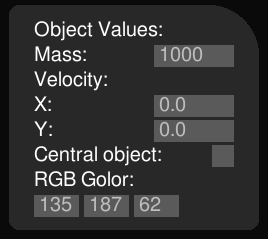
\includegraphics[width=0.5\linewidth]{p2_crop.png}
\end{center}

\emph{ObjPopup} opět dědí z třídy \emph{UI}. V konstruktoru se předem definují
všechny popisky a jejich počáteční pozice vůči levému hornímu rohu widgetu,
samotné vstupy se musí generovat vždy při první vykreslení, protože počáteční
hodnoty musí vždy odpovídat libovolnému zvolenému objektu. 

\paragraph{Draw}
Funkce \emph{Draw} této třídy přijímá jako další argument objekt, se kterým
uživatel zrovna pracuje. Ten si udržuje po celou dobu, kdy je widget otevřený.
Dále se zde předdefinuje poloha na obrazovce, kde se bude vykreslovat. Jak
již bylo řečeno při prvním vykreslení, se musí založit všechny vstupy se
správnymi hodnotami. O to se stará následující funkce \emph{SetupInput}, kde je
pevně vytvořené nastavení všech vstupů, pouze se doplní potřebné vlastnosti
zpracovávaného objektu. Tato třída nevyužívá jako pozadí svého widgetu obrázek,
proto ve své vykreslovací funkci ještě vytváří vlastní vzhled pozadí,
vykreslené pod vstupy. Dále se potřebné proměnné předávají do původní zděděné
\emph{Draw} funkce pro vykreslování popisků a vstupů.

\paragraph{Event\underline{ }handler}
Toto je nejrozsáhlejší metoda této třídy. Pracuje s logikou všech vstupních
prvků, kontroluje správnost vstupů a zpracovává jejich \\propojení s upravovaným
objektem. Podrobněji ve vlastních komentářích v kódu.
\\
\subsubsection{Třída InputField}
\paragraph{}
Tato třída je pomocná hlavnímu widgetu. Vytváří textové pole (preferovaný je
číselný vstup), s pomocnou kontrolou správnosti vložených hodnot. Důležitou
proměnnou v konstruktoru je \emph{pointer}, specifikující kterou hodnotu vstup
upravuje.

\paragraph{Draw}
Vykreslovací metoda této třídy je poměrně jednoduchá. Nejprve dle podmínek volí
barvu textu, poté vytváří a vykresluje vlastní textový řetězec.

\paragraph{SetText}
Funkce \emph{SetText} je klasický hodnotový setter s vlastní kontrolou
zapisovaných dat. Pro toto využití je nejdůležitější možnost vytvořit limity,
kterými se výstupy daného pole musí řídit.

\paragraph{GetDragValue}
Tato funkce tvoří ovládání pro změnu hodnot textového pole, pomocí tažení
kurzoru. Uživatel může kliknout a držet textové pole a pohybem myši do
libovolné strany, hodnotu zvyšovat/zmenšovat.

\newpage
\subsubsection{Třída RadioButton}
\paragraph{}
V této třídě se definuje zaskřtávací tlačítko, které umožňuje předávat hodnoty
true/false.

\paragraph{Draw}
Metoda vykreslující tento vstup je také poměrně jednoduchá. \\Nejprve se zvolí
text (výplň) tlačítka, podle bool proměnné \emph{toggle}. Text je potom
vykreslován ve správné barvě na předem vytvořené pozadí.

\paragraph{Event\underline{ }handler}
Třída má vlastní \emph{Event\underline{ }handler}, protože jednotlivé \\vstupy je
potřeba řešit blíže na straně samotného tlačítka. Pro možný event (stisknutí
tlačítka) se zde řeší patřičné vizuální a logické změny.
\\
\subsubsection{Třída TopMenu}
\paragraph{}
\emph{TopMenu} je další třída, která přímo dědí z hlavní šablony \emph{UI}.
Využívá se pro vytváření nabídky panelu nástrojů, který je uživateli vždy
přístupný v horní části obrazovky.

\begin{center}
    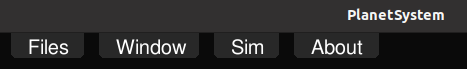
\includegraphics[width=0.9\linewidth]{p3_crop.png}
\end{center}

Toto menu má formu záložek, které se při rozkliknutí mohou otevřít do více
tlačítek, nebo do dalšího samotného okna.

\paragraph{Konstruktor}
Konstruktor této třídy dědí z původní třídy \emph{UI}, ale je navíc obohacený o
proměnné ukládající možný obsah tlačítek spadající pod danou záložku, barevný
design záložky a rozvržení velikost prostoru, ve kterém bude každá záložka pracovat.

Tyto hodnoty jsou všechny určeny k úpravě a přesnému nadefinování při vytváření
samotného ovládacího panelu v hlavní části programu.

\paragraph{Draw}
Vykreslovací funkce zde vyžaduje více proměnných, protože je potřeba zajistit
správné zarovnání záložek vedle sebe i ve chvílích, kdy můžeme v \\programu
zvolit libovolný rozměr tlačítka. Dále zde vykresluje jednotlivá tlačítka
uvnitř záložky, pokud je daná záložka rozkliknuta.

\paragraph{Event\underline{ }handler}
Vlastní \emph{Event\underline{ }handler} pak zajištuje správné změny barev při
interakci, kontroluje jestli je uživatel kurzorem stále v oblastni záložek
(pro automatické zavírání), kontroluje potřebu otevřít záložku (kliknutí), nebo
posunutí řešení eventů hlouběji do jednotlivých tlačítek záložky, pokud jsou
otevřená.

Funkce taky pro různé výsledky vrací hodnoty, které jsou potřebné do logiky
práce hlavního programu (př. záložka sama nedokáže otevřít připojené informační
menu).
\\
\subsubsection{Třída MenuItem}
\paragraph{}
Tato třída je blízce spojená s předchozí třídou. Objekty třídy \emph{MenuItem}
tvoří vnitřní části záložek, zobrazené pouze po rozkliknutí dané záložky.

\paragraph{Konstruktor}
Pro jednotlivé objekty můžeme definovat jejich vnitřní text, pointer funkce na
kterou ukazují, text možné klávesové zkratky a její pozici v tlačítku a
samotnou šířku tlačítka.

\paragraph{Draw}
Pro vykreslování funkce nejprve dopočítává správnou polohu řádku, na kterém
tlačítko bude. Poté již standardně vykreslí pozadí tlačítka a hlavní text (s
možnou zkratkou).

\paragraph{Event\underline{ }handler}
Typický vlastní \emph{Event\underline{ }handler}, nejprve zpracovává vizuální
stránku tlačítka (změny barev při přejetí kurzorem přes tlačítko), poté možné
kliknutí, po kterém by vracel hodnotu svého \emph{pointeru}.

\subsection{PlanetSystem} 
\paragraph{Úvod}
Toto je centrální část celého program, která propojuje všechny moduly a sama
provádí hlavní část výpočtů simulace prostředí. 

\paragraph{Výčet proměnných} 
V úvodu programu se nachází výčet všech proměnných (magických konstant), které
jsou využívány napříč programem. Velmi důležité jsou zejména konstanty
ovlivňující fyzikální simulaci. Důležitou proměnnou je \emph{STEPTIME}
ovlivňující kolik bude času mezi faktickými fyzikálními kroky (hodilo by se 0
vteřin, ale to pro nás není možné), menší hodnota vrací přesnější simulaci za
ceny nárůstu výpočetní síly. 

\paragraph{Hlavní cyklus aplikace} Celý běhový cyklus aplikace se nachází v
poslední části zdrojového kódu uzavřený do těla while cyklu. Ačkoli se jedná
na první pohled o nekonečný cyklus, k zacyklení nedojde kvůli ošetření
výstupů Pygame eventů, umožňující aplikaci řádně ukončit.
\\\\
Další popis bude postupovat podle pořadí průběhu typického aplikačního cyklu.

\begin{itemize}
    \setlength\itemsep{-3pt}
    \item V první fázi dochází k vyčištění obrazovky z předchozího cyklu do
        předem nastavené barvy. 

    \item Poté dochází ke kontrole, zda v seznamu simulovaných objektů není
        takový, ve kterém došlo ke změně (daný objekt nastaví svoji proměnnou
        \emph{simUpdate} na True) a tudíž by bylo potřeba simulaci přepočítat.
        Podmínka \emph{PAUSE and TIMESTEP == 0} ve své podstatě značí, že se
        stále jedná o fázi, kdy uživatel edituje objekty. Samotný výpočet
        simulace probíhá ve funkci \emph{sim}, která pro určený počet kroků
        dopředu vypočítá polohu a rychlost každého z objektů v daném kroku
        simulace.

    \item Pokračuje se vykreslením všech planetárních objektů a jejich \\trajektorií.

    \item Dále se pro potřeby ukládání souborů volá funkce, která může
        zaznamenat snímek obrazovky (důležité ještě před vykreslením UI
        elementů).
    
    \item Další je vykreslování UI - horní panel záložek a widget objetku
        (pokud je nějaký zvolen).

    \item Pokud máme z předchozích cyklů vybraný nějaký objekt a uživatel
        stisknul šipku (posouvání objektu), voláme v této chvíli metodu pro
        posun na zvolený objekt.

    \item V tomto bodě se cesta dělí na tři stavy. SIM stav pracuje v době
        vlastní simulace a editování, stav LOAD a ABOUT zastavují simulační
        cyklus a vykreslují vlastní menu.
        
        \textbf{Stav SIM}:
        \begin{itemize}
            \setlength\itemsep{0pt}
            \item Podobně jako u posunu objektu, posun kamery se řeší stejným
                způsobem. Program si pamatuje, které směrové klávesy má
                uživatel stisknuté a pro ně v dalším cyklu udělá požadovaný
                posun.
            \item Další je řešení a předávání možných eventů (stisknutí
                tlačítka myši, klávesnice, pohyb myši, ukončení aplikace,
                atd.). 
            \item Pokud jsme ve fázi editování a uživatel vybral nějaké těleso,
                eventy hlavního okna se dále posílají ke zpracování do widgetu
                (textové vstupy, tlačítka). 
            \item Stisknutí dalších kláves je posíáno do funkce
                \emph{shortcutEvents} pro zpracování vybraných podporovaných
                klávesových zkratek, které uživatel mohl využít. 
            \item Pak se také všechny možné eventy posílají jednotlivým
                záložkám horního \emph{TopMenu} pro vlastní zpracování.
            \item Další jsou samostatně zpracovávané eventy spojené s kliknutím
                tlačítka myši, scrollování kolečka myši, pohyb pomocí kláves
                WSAD (kamera) a pohyb pomocí šipek (tělesa). 
            \item Poslední část v SIM stavu zajišťuje, že spuštěná simulace
                vždy poběží co nejpřesněji ve zvoleném FPS (rychlosti). Vlastní
                Pygame cyklus je nepřesný a při vyšší zátěži je jeho délka
                proměnlivá. Proto je v tomto programu vedlejší hodnota
                počítající simulační cykly, která je nezávislá na rychlosti
                Pygame (pouze na reálném čase).
        \end{itemize}

        \textbf{Stav LOAD}:
        \begin{itemize}
            \item Při tomto stavu se zastaví všechny fyzikální výpočty a
                vykreslování a logika spojená s Pygame eventy se přesune do
                funkce \\\emph{loadDrawing}. Zde je uživatel schopen načíst zpět
                své dříve uložené simulace.
        \end{itemize}

        \textbf{Stav ABOUT}:
        \begin{itemize}
            \item Podobně jako u LOAD, všechno vykreslování se přesouvá do
                funkce \emph{aboutDrawing}. Ta vykresluje hlavní informační
                text v aplikaci. Text samotný nemá žádnou přidanou logiku,
                která by řešila Pygame eventy, tudíž pro možné ukončení
                aplikace je přímo do tělesa \\tohoto stavu přidáno možnost
                ukončení aplikace (LOAD tento stav řeší sám).
        \end{itemize}

    \item Poslední částí jsou funkce Pygame, vykreslující připravenou grafiku
        do okna pro uživatele a opakování cyklu v čase zvoleném ve funkci
        \emph{tick} (60 = FPS).
\end{itemize}

\newpage
\section{Ukládání souborů}
\paragraph{}
\emph{LOAD} menu nabízí uživateli možnost své simulace ukládat a znovu načítat.
Tato funkce pracuje s externí složkou "\emph{.saves}" ukrytou ve složce s
\\programem. Pro správnou funkčnost se musí při ukládání zachovat určitá
struktura. 

Při ukládání se vytvoří pomocí knihovny \textbf{Pickle} soubor se všemi daty
simulace a dalšího nastavení a pomocí vlastní screenshot funkce se zaznamená
jak vypadá aktuální obrazovka. Oba dva soubory se uloží do složky "\emph{.saves}".

Data simulace jsou uložené v souboru typu "save\underline{ }\#.sim" a snímek \\obrazovky
"sImg\underline{ }\#.png". Z programátorského hlediska, ve fázi vývoje \\mohou být jména
souborů externě změněna do tvaru "preset\underline{ }\#.sim" a "pImg\underline{ }\#.png". Tyto soubory
pak \emph{LOAD} funkce vnímá jako defaultní příklady a pro tyto uložené
simulace pak nebude nabízena možnost soubor vymazat.
\\
\section{Možnosti dalšího rozvoje}
Ačkoli se již jedná o plnou, funkční verzi programu, jsou jistě věci, které
bych osobně rád dodělávál a vylepšoval i nadále. Vedle celkové optimalizace
\\(rychlejší funkčnost pro uživatele, jiný platforma než Python) by se řadila
ještě třeba lokalizace jazyků, úprava celkového UI designu a zajištění co možná
nejšiřší kompatibility bez ztráty funkčnosti. 
\\\\
\end{document}
